
\section{Dataflow parallelism and map-reduce computing}
\label{sec:background}

Today's data-intensive computing derives much from earlier work on
parallel databases.  Broadly speaking, data is read from input files,
processed, and stored in output files.  The dataflow is organized as a
pipeline in which the output of one operator is the input of the
following operator.  DeWitt and Gray \cite{paralleldatabases} describe
two forms of parallelism in such dataflow systems: partitioned
parallelism and pipelined parallelism.  Partitioned parallelism is
achieved by partitioning the data and splitting one operator into many
running on different processors.  Pipelined parallelism is achieved by
streaming the output of one operator into the input of another, so
that the two operators can work in series on different data at the
same time.

Google's MapReduce\footnote{We refer to the programming model as map-reduce
and to Google's implementation as MapReduce.} \cite{mapreduce} offers a
simple programming model that facilitates development of scalable parallel
applications that process a vast amount of data.
% on clusters of commodity machines.
Programmers specify a {\it map} function that generates values and
associated keys from each input data item and a {\it reduce} function
that describes how all data matching each key should be combined.
The runtime system handles details of scheduling, load balancing, and
error recovery.
Hadoop \cite{hadoop} is an open-source implementation of the map-reduce model.
Figure \ref{fig:mapreduce} illustrates the pipeline of a map-reduce
computation involving three nodes (computers).
The computation is divided into two phases, labeled Phase 1 and Phase 2.

%TODO: Jay recommends adding partitioned and pipelined parallelism
%with a graph annotation
{
\renewcommand{\baselinestretch}{1.0}
\begin{figure}[t]
\begin{center}

\resizebox{\columnwidth}{!} {
   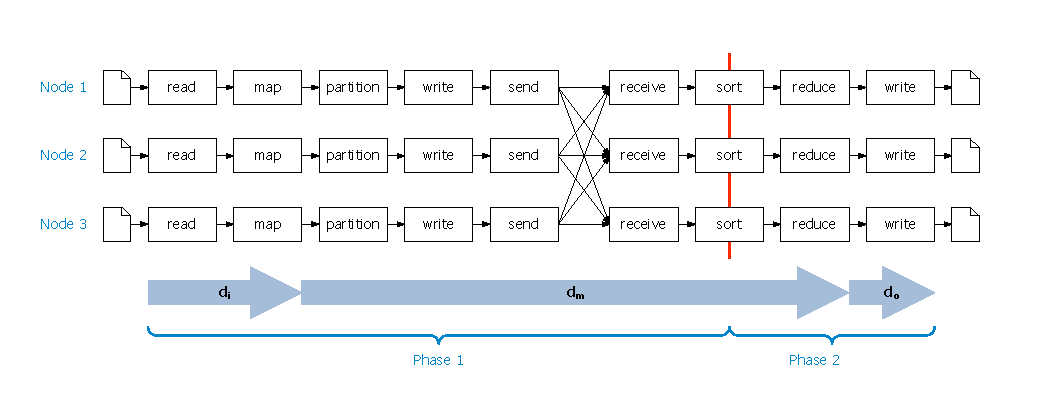
\includegraphics[width=6in]{fig_mapreduce_dataflow.eps}
}

\end{center}
\minicaption{A map-reduce dataflow}

\label{fig:mapreduce}
\end{figure}
}


\minorsection{Phase 1}
Phase 1 begins with the reading of the input data from disk and ends with the
sort operator. It includes the map operators and the exchange of data over the
network.
The first write operator in Phase~1 stores the output of the map operator.
This ``backup write'' operator is optional, but used by default in the
Google and Hadoop implementations of map-reduce, serving to increase the
system's ability to cope with failures or other events that may occur later.

\minorsection{Phase 2}
Phase 2 begins with the sort operator and ends with the writing of the output
data to disk. In systems that replicate data across multiple nodes,
such as the GFS \cite{gfs} and HDFS \cite{hdfs} distributed file systems
used with MapReduce and Hadoop, respectively, the output data must be sent
to all other nodes that will store the data on their local disks.

\minorsection{Parallelism}
In Figure \ref{fig:mapreduce},
partitioned parallelism takes place on the vertical axis;
the input data is split between three nodes, and each operator
is, in fact, split into three sub-operators that each run on a different node.
Pipelined parallelism takes place on the horizontal axis;
each operator within a phase processes data units (e.g., records) as it
receives them, rather than waiting for them all to arrive, and passes data
units to the next operator as appropriate.
The only breaks in pipelined parallelism occur at the boundary between phases.
As shown, this boundary is the sort operator.
The sort operator can only produce its first output record after it has
received all of its input records, since the last input record received
might be the first in sorted order.
%May want to add citation to work eliminating barrier

\minorsection{Quantity of data flow}
Figure \ref{fig:mapreduce} also illustrates how the amount of data ``flowing''
through the system changes throughout the computation. The amount of input data
per node is $d_i$, and the amount of output data per node is $d_o$. The amount
of data per node produced by the map operator and consumed by the reduce
operator is $d_m$. In most applications, the amount of data flowing through the
system either remains the same or decreases (i.e., $d_i \ge d_m \ge d_o$). 
In general, the mapper will implement some form of select, filtering out
rows, and the reducer will perform aggregation.  This reduction in data across the stages can play a key
role in the overall performance of the computation.  Indeed, Google's
MapReduce includes ``combiner'' functions
%\footnote{To the extent that
% we model combiner functions it is in the amount of data the mapper's
% output}
to move some of the aggregation work to the map operators and, hence,
reduce the amount of data involved in the network exchange~\cite{mapreduce}.
Many map-reduce workloads resemble a ``grep''-like computation, in which the map operator decreases
the amount of data ($d_i \gg d_m$ and $d_m = d_o$).
In others, such as in a sort, neither the map nor the reduce
function decrease the amount of data ($d_i = d_m = d_o$).

%the read
%operator reads the data from
%disk as a stream, so each record that is read from disk can be immediately
%passed to the map operator, which can convert (i.e., ``map'') that record into
%zero or more records that are then passed to the partition operator, and so
%forth. In other words, the map operator does not need to wait for all of the
%input to be read from disk, and the partition operator does not need to wait
%for the map operator to finish operating on all of the records.

%\fix{Need to talk about the optional backup write here, so it makes
%sense later in the model.  I see some commented out info on that here...}

%Without this mechanism, all map tasks must be re-executed if a single
%reduce task stops running.
%When running a long computation on a large cluster, where it is
%likely that one of the tasks will stop running during the computation, it is a
%good idea to include this step.  However, if the total number of ``machine
%hours'' required for a computation is small, the performance benefit from
%omitting this step probably outweighs the cost of having to re-run the
%computation if one of the tasks stops running during the original
%computation.

\subsection{Related work}
\label{sec:related_work}

Concerns about the performance of map-reduce style systems emerged
from the parallel databases community, where similar data processing
tasks have been tackled by commercially available systems. In
particular, Stonebraker et al.\ compare Hadoop to a variety of DBMSs
and find that Hadoop can be up to 36x slower than a commercial
parallel DBMS~\cite{stonebraker-mr}.  In previous
work~\cite{efficiencymatters}, two of the authors of our paper pointed
out that many parallel systems (especially map-reduce systems, but
also other parallel systems) have focused almost exclusively on
absolute throughput and high-end scalability.  This focus, as the
authors quantify by back-of-the-envelope comparisons, has been at the
detriment of other worthwhile metrics.
%Another author of this
%paper describes the analytical model in~\cite{tshiranthesis}.

In perhaps the most relevant prior work, Wang et al.\ use simulation
to evaluate how certain design decisions (e.g., network layout and data
locality) will effect the performance of Hadoop
jobs~\cite{mr-simulation}.  Specifically, their MRPerf simulator
instantiates fake jobs, which impose fixed times (e.g., job startup)
and input-size dependent times (cycles/byte of compute) for the Hadoop
parameters under study. The fake jobs generate network traffic
(simulated with ns-2) and disk I/O (also simulated).  Using execution
characteristics accurately measured from small instances of Hadoop
jobs, MRPerf accurately predicts (to within 5-12\%) the performance
of larger clusters.  Although simulation techniques like MRPerf are
useful for exploring different designs, by relying on measurements of
actual behavior (e.g., of Hadoop) such simulations will also emulate any
inefficiencies particular to the specific implementation simulated.

%DISC~\cite{disc}

%Efficiency matters~\cite{efficiencymatters} and Tomer's thesis~\cite{tshiranthesis}.

%MapReduce~\cite{mapreduce}, GFS~\cite{gfs}, Hadoop~\cite{hadoop}, HDFS~\cite{hdfs}, Dryad~\cite{dryad}.

%The language integration and translation to an execution plan has an
%effect on performance~\cite{distagg}.  Dryad LINQ~\cite{dryadlinq} and
%Pig latin~\cite{piglatin} provide higher-level SQL-like languages for
%expressing and automatically optimizing programs on a given system.

%DataSeries~\cite{dataseries} and Sawzall~\cite{sawzall}.

%Gordon~\cite{gordon} and FAWN~\cite{fawn}.

%Parallel database systems~\cite{paralleldatabases}, and Phoenix~\cite{phoenix}.

%Raid~\cite{raid}
